\mychapter{Modelling}{Modelling}{}
\label{chap:modelling}

\mysection{Introduction}{Introduction}
\label{sec:modintro}

This project focuses on the pose estimation of a satellite using satellite images. This is essentially a localistion problem
and requires a realistic description of the system. The aim of this chapter is to sufficiently define the problemand the proposed solution. Estimation
algorithms is discussed and an estimator is chosen to solve the localisation problem. Further, attitude representations of a rigid body is introduced
along with the dynamic and kinematic models used to describe a satellite in inertial space. Attention is given to quaternion attitude representations along
with their propagation using angular rates.

\mysection{Problem Definition}{Problem Defintion}
\label{sec:moddef}

A satellite orbiting Earth in the Earth-Centered Inertial (ECI) reference frame performs Earth observation missions, 
continuously capturing high-resolution imagery of the planet's surface for scientific, commercial, or operational purposes. 
To fulfill mission objectives effectively, the satellite must provide not only high-quality imagery but also precise geographic 
information about observed areas. This requires accurate knowledge of the satellite's six-degree-of-freedom pose 
(three-dimensional position and three-dimensional attitude) relative to the ECI frame at the moment each image is captured.
\vspace{0.5cm}

Traditional satellite pose determination relies on external systems such as Global Navigation Satellite Systems (GNSS) 
and ground-based tracking networks. However, this thesis investigates an autonomous approach where the satellite performs 
"visual navigation" by identifying known ground features in its imagery and using these observations to determine its orbital 
state. The satellite essentially performs "reverse GPS" - instead of receiving position signals from space, it observes 
recognizable landmarks on Earth's surface and computes its pose from these visual references.
\vspace{0.5cm}

The core technical challenge lies in the transformation from raw imagery to precise pose estimates. This involves several 
interdependent problems: \textbf{(1) Feature Detection} - identifying which pixels in the imagery correspond to cataloged 
landmarks among millions of pixel observations; \textbf{(2) Geometric Inversion} - solving the complex inverse problem of 
determining six-dimensional pose from two-dimensional image projections of three-dimensional landmarks with known geographic 
coordinates; and \textbf{(3) Uncertainty Management} - handling measurement noise, feature detection errors, and dynamic orbital 
motion in real-time. This thesis assumes the availability of a pre-established catalog of ground features with precisely 
known geographic coordinates in the ECI frame. The feature matching problem - associating detected image features with specific 
catalog entries - is considered solved through prior knowledge of the observed terrain and existing geographic databases.
\vspace{0.5cm}

\begin{figure}[htbp]
    \centering
    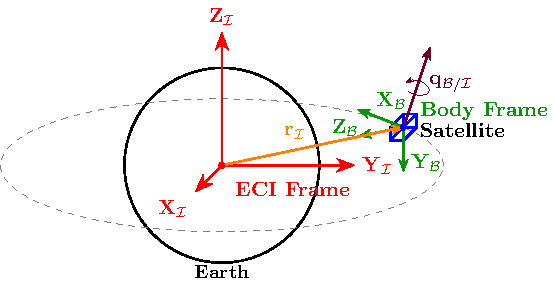
\includegraphics[width=0.8\textwidth]{figures/Figure1.pdf}
    \caption{Satellite pose estimation concept showing orbital geometry, reference frames}
    \label{fig:satellite_concept}
\end{figure}

This problem structure aligns with a simplified version of the Simultaneous Localization and Mapping (SLAM) framework. 
In this context, \textbf{localization} corresponds to determining the satellite's pose relative to the ECI frame using 
observations of cataloged features, while the \textbf{mapping} component is reduced to feature catalog utilization rather 
than creation. Since the geographic locations of observable features are assumed known a priori, the primary focus becomes the 
pose estimation problem given established feature correspondences.
\vspace{0.5cm}

The satellite's pose estimation system must account for the dynamic nature of orbital motion, 
the geometric relationship between the camera frame and satellite body frame, and the projection 
characteristics of the imaging system, while maintaining computational efficiency suitable for 
real-time onboard processing. 

%=============================================================================================================================================================================

\mysection{Refrence Frame Transformations}{Refrence Frame Transsformations}

In this masters we are going to encounter a few different refrence frames. To accurateley to create the measurement model we should have an understanding of all the different 
reference models and how to transform from one to another

\mysubsection{Lattitude, longitude and altitude}{Lattitude, longitude and altitude}

The lattitude, longitude of a feature or the position of the satellite is donated with the $\mathcal{L}$. The lattitude of a feature is the position of how high or low it above the
equator, having a range of $-90^{\circ}$ to $90^{\circ}$. The longitude is based of the greenwich maridian, a longitude line that pases through the north- and south pole, it has a
range of $-180^{\circ}$ to $180^{\circ}$. The altitude is measured form the the "WGS84" elliptical globe.

\begin{equation}
    \mathbf{r}_\mathcal{L} = \begin{bmatrix}
    \lambda \\
    \phi \\
    h    
    \end{bmatrix} 
\end{equation}

\mysubsection{Earth Ceneterd Earth Fixed}{Earth Ceneterd Earth Fixed}

The Earth Ceneterd Earth Fixed refrence frame is represented by the $\mathcal{F}$ and is very simular to the $\mathcal{L}$ reference frame with the z-axis alligned with the northpole
and the x-axis points at the crossing of the Prime Maridian an the Equator, where the y-axis completes the right hand rule. The x,y and z-axis is defined in kilometers.
To covert from $\mathcal{L}$ to $\mathcal{F}$ is to use a "WGS84" transfomr. Where WGS84 stands for World Geodetic System 1984, which is the standard coordinate system used for
Global Positioning System (GPS). The WGS84 transformation uses a reference ellipsoid that uses a semi-major axis of 6,378 km and a flatting of 1/298.2 .

\begin{equation}
        \mathbf{A}_{\mathcal{L}}^{\mathcal{F}} = f(\text{WGS84})
\end{equation}

\begin{figure}[H]
    \centering
    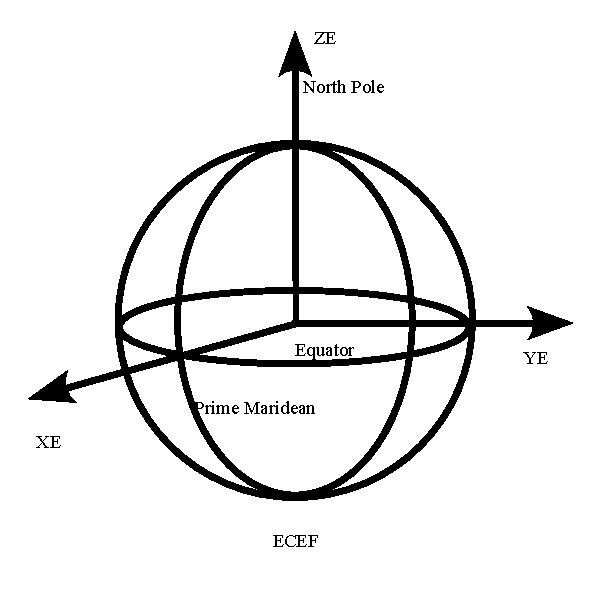
\includegraphics[width=0.4\textwidth]{figures/modelling/ECEF.pdf}
    \caption{This figure represents the Earth Ceterned Earth Fixed reference frame with the X-axis defined in the direction of the equator and primemaridean
    with z-axis defined as the north pole and the y-axis completing the right had rule.}
    \label{fig:ECEFRF}
\end{figure}

\mysubsection{Earth Ceneterd Inertial}{Earth Ceneterd Inertial}

The Earth Centered Inertial refrence fream (ECI) refrenced by $\mathcal{I}$ shares a refrence frame axis with the ECEF, but is rotated about the z-axis. This rotation is governed
by the rotation speed of the earth $\omega_e$ which is $7.2921\times10^{-5}$ rad/s and time $t$. To transform from the ECEF reference frame to the ECI reference frame one should
rotate the Earth clockwise e.i. 

\begin{equation}
    \mathbf{A}_{\mathcal{F}}^{\mathcal{I}} = R(\omega_e t) = 
    \begin{bmatrix}
        \cos(-\omega_e t) & -\sin(-\omega_e t) & 0\\
        \sin(-\omega_e t) & \cos(-\omega_e t) & 0\\
        0 & 0 & 1
    \end{bmatrix}
\end{equation}

\begin{figure}[H]
    \centering
    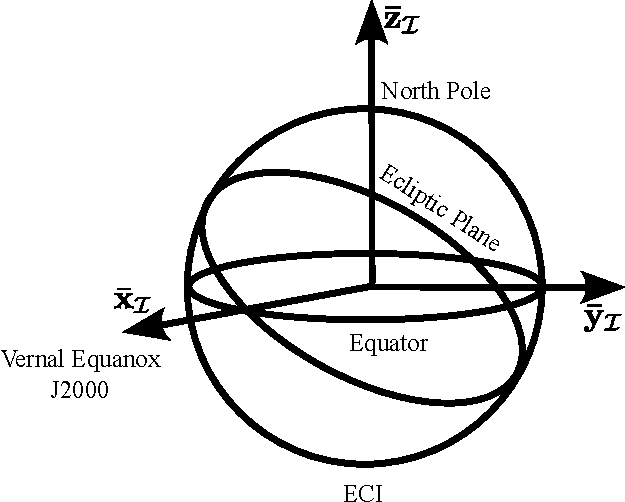
\includegraphics[width=0.4\textwidth]{figures/modelling/ECI.pdf}
    \caption{This figure represents the Earth Centered Inertial Reference frame with the x-axis defined in the direction of the vernel equanox, which is the defined as the crossing
    of the ecliptic plane and the eqautor, the z-axis is defined as the north pole and the y-axis completes the rght hand rule.}
    \label{fig:ECIRF}
\end{figure}

\mysubsection{Orbital reference frame}{Orbital reference frame}

The orbital reference frame used is the Local Vertical Local Horizon (LVLH) denoted by $\mathcal{O}$. \textcolor{red}{The LVLH frame is a rotating, orbit-attached corrdinate
system commonly used in spacecraft dynamics. It moves with the satellite and is defined relative to its orbit around Earth}. The x-axis is the "Local Horizon" also called
"along track" pointing forward it is tangent to the orbit and points in the direction of motion. The z-axis is the local vertical and is also called the Nadir direction, it points
to the barycenter of the system, in this case the center of the Earth. The y-axis is called the cross track it completes the right handed system. It points out of the orbital plane,
typically the angular momentum vector direction (normal to the orbit plane).

if $\mathbf{r}$ is the position vector of the satellite and $\mathbf{v}$ is the velocity vector of the satellite.
The equation for the reference frame is:

\begin{align}
    \bar{z}_{\mathcal{O}} &= -\frac{\mathbf{r}}{||\mathbf{r}||} \\
    \bar{y}_{\mathcal{O}} &= \frac{\mathbf{r}\times\mathbf{v}}{||\mathbf{r}\times\mathbf{v}||}\\
    \bar{x}_{\mathcal{O}} &= \bar{y}_{\mathcal{O}}\times\bar{z}_{\mathcal{O}}
\end{align}

For this reference frame there should also be a refrence frame translation introduced. Which is done by substracing $\mathbf{r}$ from the vector

\begin{equation}
    \mathbf{f}_{\mathcal{O}} = \mathbf{A}_{\mathcal{I}}^{\mathcal{O}}\times(\mathbf{f}_{\mathcal{I}} - \mathbf{r}_{\mathcal{I}})
\end{equation}

\begin{figure}[H]
    \centering
    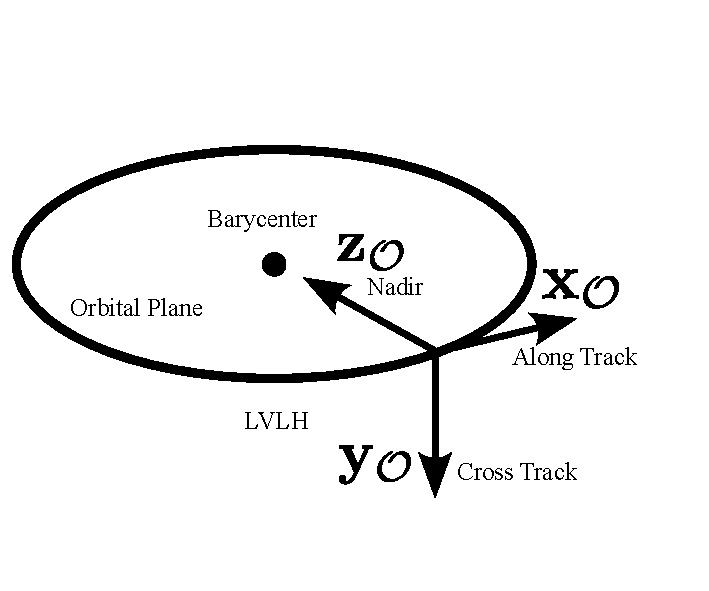
\includegraphics[width=0.4\textwidth]{figures/modelling/LVLH.pdf}
    \caption{This figure represent the Local Vertical Local Horizon Referenece frame, more commonly refered to as the orbitial refrence frame. In the orbitial refrence frame
    the z-axis is defined as Nadir, meaning that it always points to the center of mass perfectly parallel to the oribital plane, the x-axis is defined as the vector tangentail
    to the plane, also known as the along track vector, and y is the completion of the right hand rule.}
    \label{fig:LVHLRF}
\end{figure}

\subsection{Body Referenece frame}

The body reference frame denoted by $\mathcal{B}$ is the reference frame of the satellite body itself, with the center point referenced as the center of mass of the satellite body.
with the z-axis defined as the yaw, x-axis defined as the roll and the y-axis defined as the pitch of the satellite. With the body frame z-axis and the orbital reference frame 
as alligned at initialisiation


\begin{figure}[H]
    \centering
    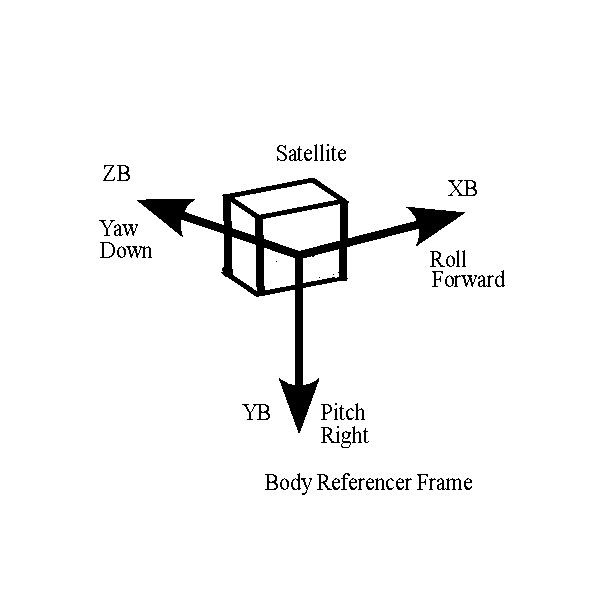
\includegraphics[width=0.4\textwidth]{figures/modelling/BRF.pdf}
    \caption{}
    \label{fig:BRF}
\end{figure}

\mysubsection{Camera Reference Frame}{Camera Reference Frame}

The camera refrence frame denoted by $\mathcal{C}$. In many Earth Observation missions the camera has its own reference frame defined relative to the Earth. Where the x-axis is
pointing directly to the Earth's surface indicatting the cameras roll axis, with the y-axis representing the pitch axis represents an angle ahead or behind of the orbit and the
z-axis representing the yaw axis.


\begin{figure}[H]
    \centering
    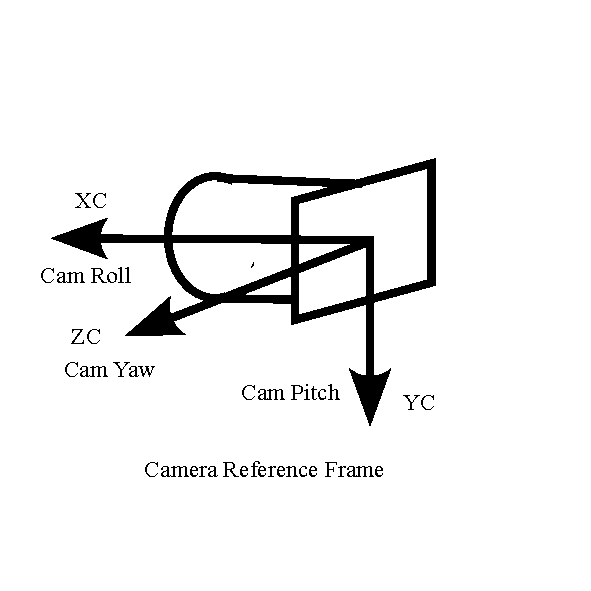
\includegraphics[width=0.4\textwidth]{figures/modelling/CRF.pdf}
    \caption{}
    \label{fig:CRF}
\end{figure}

\begin{equation}
    \mathbf{f}_{\mathcal{C}} = \mathbf{A}_{\mathcal{O}}^{\mathcal{C}}\times\mathbf{f}_{\mathcal{O}}
\end{equation}

\mysubsection{Image Reference Frame}{Image Reference Frame}

\begin{figure}[H]
    \centering
    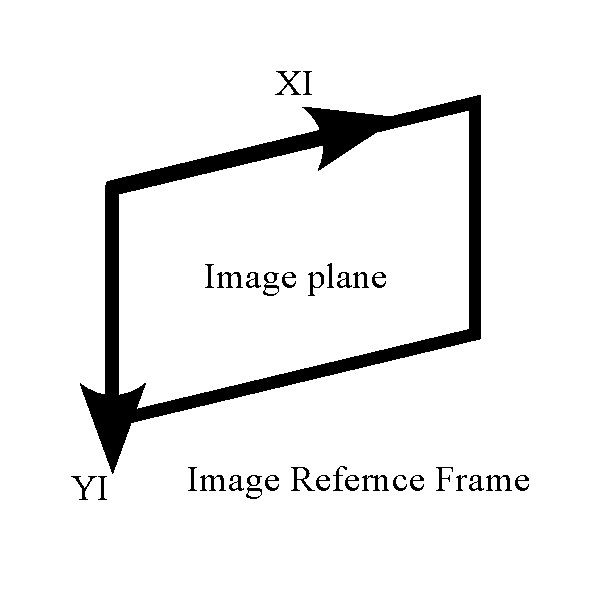
\includegraphics[width=0.4\textwidth]{figures/modelling/MRF.pdf}
    \caption{}
    \label{fig:MRF}
\end{figure}


\mysubsection{East - North - Up}{East - North - Up}


%==================================================================================================================================================================================

\mysection{Rigid Body Mechanics}{Rigid Body Mechanics}
\label{sec:modrigid}

\mysubsection{Kinematics}{Kinematics}
\label{sec:kinematics}

\textcolor{red}{The pose of a rigid body in a refrence frame consists of the position and attitude of the body. The attitude, or orientation of a body-fixed reference frame to a
known reference frame. This is usualy represented by a rotation matrix, often referred to as a direction cosine Matrix (DCM). A rotation about a single coordinate axis
is referred to as a coordinate rotation. A coordinate rotation about the x-,y- and z-axes with angles $\phi$, $\theta$ and $\psi$, of the body can be respectivley
describes as, [Willem de Jong p.23]}

\begin{equation}
    R_x(\phi) = \begin{bmatrix} 
        1 & 0 & 0 \\
        0 & \cos(\phi) & \sin(\phi) \\
        0 & -\sin(\phi) & \cos(\phi)
    \end{bmatrix}
    \label{Eq:3.1}
\end{equation}

\begin{equation}
    R_y(\theta) = \begin{bmatrix} 
        \cos(\phi) & 0 & -\sin(\phi) \\
        0 & 1 & 0 \\
        \sin(\phi) & 0  & \cos(\phi)
    \end{bmatrix}
    \label{Eq:3.2}
\end{equation}

\begin{equation}
    R_z(\psi) = \begin{bmatrix} 
        \cos(\phi) & \sin(\phi) & 0 \\
        -\sin(\phi) & \cos(\phi) & 0 \\
        0 & 0 & 1
    \end{bmatrix}
    \label{Eq:3.3}
\end{equation}

\textcolor{red}{Any rotation in 3D space can be described by three coordinate rotations. The DCM describing the attitude of the target in the camera reference frame
(CRF), $\mathbf{A}_{\mathcal{C}}^{\mathcal{B}}$, can be represented by three Eular angles. Each of the angles corresponds to one coordinate rotation. The order
of the Eular 1-2-3 rotation, shown in Figure 3.5, is expressed as}

\begin{equation}
    \boldsymbol{A}_{\mathcal{C}}^{\mathcal{B}} = R_x(\phi)R_y(\theta)R_z(\psi)
    \label{Eq:3.4}
\end{equation}

\begin{equation}
    \begin{bmatrix}
        a_{1,1} & a_{1,2} & a_{1,3}\\
        a_{2,1} & a_{2,2} & a_{2,3}\\
        a_{3,1} & a_{3,2} & a_{3,3}\\
    \end{bmatrix}
\end{equation}

\begin{equation}
    \begin{bmatrix}
        C\theta C\psi & C\theta S\psi &  -S\theta\\
        S\phi S\theta C\psi - C\phi S\psi & S\phi S\theta S\psi + C\phi C\psi & S\phi C\theta\\
        C\phi S\theta C\psi + S\phi S\psi &  C\phi S\theta S\psi - S\phi C\psi & C\phi C\theta
    \end{bmatrix}
\end{equation}

\textcolor{red}{Where S is the sine function and C is the cosine function. The Eular angles are calculated as follows}

\begin{equation}
    \phi = \arctan2\left(\frac{a_{2,3}}{a_{3,3}}\right)
\end{equation}

\begin{equation}
    \theta = \arctan2\left(\frac{-a_{1,3}}{\sqrt{a_{1,1}^2} + \sqrt{a_{1,2}^2}}\right)
\end{equation}

\begin{equation}
    \psi = \arctan2\left(\frac{a_{1,2}}{a_{1,1}}\right)
\end{equation}

\textcolor{red}{mathematicl singularities occur when using Eular angles to represent large rotations. When both $a_{1,1}$ and $a_{1,2}$ in Equation \ref{Eq:3.4} are zero, the expressions
for $\psi$ and $\theta$ ar undefined. This is known as \textit{gimbal lock}, where the changes in the first and third Eular angles are indistinguishable when the second angle nears
a criticual value. Alternatively, the DCM can be described using quaternions, which do not have these singularities. The quaternion rotation is Figure ?? is expressed by the Eular axis
$\mathbf{\bar{e}}=[e_x,e_y,e_z]^T$ and the angle $\theta$}

\begin{equation}
    \mathbf{q} = \begin{bmatrix} q_s \\ q_x \\ q_y \\ q_z \end{bmatrix}
    = \begin{bmatrix} \cos(\theta/2) \\ e_x\sin(\theta/2) \\ e_y\sin(\theta/2) \\ e_z\sin(\theta/2) \end{bmatrix}
\end{equation}

\begin{figure}[H]
    \centering
    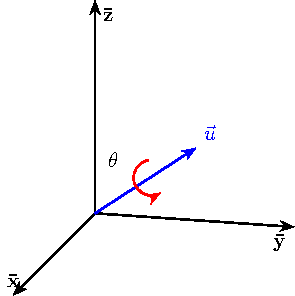
\includegraphics[width=0.3\linewidth]{figures/Quaternion.pdf}
    \caption{Quaternion Rotation}
    \label{fig:3.2}
\end{figure}

\textcolor{red}{The DCM as a function of Quaternion set is expressed as,}

\begin{equation}
    \mathbf{A}_{\mathcal{C}}^{\mathcal{B}} = 
    \begin{bmatrix}
    q_s^2 + q_x^2 - q_y^2 - q_z^2 & 2(q_x q_y - q_s q_z) & 2(q_x q_z + q_s q_y) \\
    2(q_x q_y + q_s q_z) & q_s^2 - q_x^2 + q_y^2 - q_z^2 & 2(q_y q_z - q_s q_x) \\
    2(q_x q_z - q_s q_y) & 2(q_y q_z + q_s q_x) & q_s^2 - q_x^2 - q_y^2 + q_z^2   
    \end{bmatrix}
\end{equation}

\textcolor{red}{Using the normalisation constraint, $q_s^2 + q_x^2 + q_y^2 + q_z^2 = 1$, the DCM Simplifies to,}

\begin{equation}
    \mathbf{A}_{\mathcal{C}}^{\mathcal{B}} = 
    \begin{bmatrix}
    1 - 2(q_y^2 + q_z^2) & 2(q_x q_y - q_s q_z) & 2(q_x q_z + q_s q_y) \\
    2(q_x q_y + q_s q_z) & 1 - 2(q_x^2 + q_z^2) & 2(q_y q_z - q_s q_x) \\
    2(q_x q_z - q_s q_y) & 2(q_y q_z + q_s q_x) & 1 - 2(q_x^2 + q_y^2)   
    \end{bmatrix}
\end{equation}

\textcolor{red}{The body-fixed angular rates of the satellite in CRF, $\mathbf{\omega}_{\mathcal{C}}^{\mathcal{B}}$, is expressed as a function of qauternions by,}

\begin{equation}
    \mathbf{\omega}_{\mathcal{C}}^{\mathcal{B}} = 
    \begin{bmatrix}
        \omega_{bx} \\ \omega_{by} \\ \omega_{bz}
    \end{bmatrix}
    = 2
    \begin{bmatrix}
       -q_x & q_s & -q_z & q_y \\
       -q_3 & q_4 & q_1 & -q_2 \\
       -q_4 & -q_3 & q_2 & q_s 
    \end{bmatrix}
    \begin{bmatrix}
        \dot{q_s} \\ \dot{q_x} \\ \dot{q_y} \\ \dot{q_z}
    \end{bmatrix}
\end{equation}

\textcolor{red}{Inversly the quaternion rates as a function of the body rates are,}

\begin{equation}
    \begin{bmatrix}
        \dot{q_s} \\ \dot{q_x} \\ \dot{q_y} \\ \dot{q_z}
    \end{bmatrix}
    =
    \frac{1}{2}
    \begin{bmatrix}
        0 & -\omega_{bx} & -\omega_{by} & -\omega_{bz}\\
        \omega_{bx} & 0 & \omega_{bz} & -\omega_{by}\\
        \omega_{by} & -\omega_{bz} & 0 & \omega_{bx}\\
        \omega_{bz} & \omega_{by} & -\omega_{bx} & 0 
    \end{bmatrix}
    \begin{bmatrix}
        q_s \\ q_x \\ q_y \\ q_z
    \end{bmatrix}
\end{equation}

\textcolor{red}{Quaternions will be used throughout this thesis for attitude representations. Quaternions do not have ambiguity regarding the order of rotations
and the rotation is around a well-defined axis. The sin and cosine elements of the rotation matrix are already encodedin the quaternion form of the DCM. Therfore,
only one matrix operation is required for attitude transforms, where Eular angles reguire three.}

%=====================================================================================================================================================================================

\mysubsection{Dynamics}{Dynamics}
\label{sec:dynamics}

The rotational dynamics of a rigid body satellite can be described using the Newton-Euler equations, 
which are applicable to all rigid inertial bodies . The angular momentum of the satellite is expressed as:

\begin{equation}
\dot{\mathbf{H}} = \frac{d\mathbf{H}}{dt} = \mathbf{I}\dot{\boldsymbol{\omega}}
\end{equation}

\noindent where $\mathbf{H}$ represents the angular momentum vector and $\mathbf{I}$ is the diagonalized moment of 
inertia tensor about the satellite's principal axes. In the absence of external torques, the rotational kinematics 
of a rigid satellite about its center of mass can be described by Euler's rotational equations:

\begin{align}
I_{xx}\dot{\omega}_x &= \omega_y\omega_z(I_{yy} - I_{zz}) \\
I_{yy}\dot{\omega}_y &= \omega_x\omega_z(I_{zz} - I_{xx}) \\
I_{zz}\dot{\omega}_z &= \omega_x\omega_y(I_{xx} - I_{yy})
\end{align}

\noindent where $I_{xx}$, $I_{yy}$, and $I_{zz}$ are the principal moments of inertia, which remain constant and 
depend on the satellite's mass distribution and geometric configuration. 

The stability characteristics of the satellite's rotational 
motion are governed by its mass distribution. According to Marsden and Ratiu , rotation about the major and minor principal 
axes is inherently stable, while rotation about the intermediate axis exhibits unstable behavior. Under constant energy conditions, any 
initial rotation about the intermediate axis will gradually redistribute energy to the major and minor axes through nutation effects.

For the translational dynamics, Newton's second law governs the linear motion of the satellite with mass $m$. The discrete-time position and velocity propagation equations are:

\begin{align}
\mathbf{r}_t &= \mathbf{r}_{t-1} + \mathbf{v}_t\Delta t + \frac{1}{2m}\mathbf{F}(t)\Delta t^2 \\
\mathbf{v}_t &= \mathbf{v}_{t-1} + \frac{1}{m}\mathbf{F}(t)\Delta t
\end{align}

\noindent where $\mathbf{F}(t)$ represents the net external force acting on the satellite. For the orbital environment 
considered in this work, where external perturbations are negligible compared to gravitational forces, and given that 
precise mass properties may not be available, the translational motion can be approximated using kinematic models where 
the current velocity depends primarily on the previous velocity state.

To propagate the quaternion representing the satellite's attitude over time, the quaternion derivative must first be computed.
 The time derivative of the quaternion $\mathbf{q}_{B/I}$, which describes the rotation from the inertial frame to the body frame,
is calculated using quaternion multiplication with the angular velocity vector:

\begin{equation}
\dot{\mathbf{q}}_{B/I} = \frac{1}{2}(\mathbf{q}_{B/I} \otimes \boldsymbol{\omega})
\end{equation}

\noindent where $\boldsymbol{\omega} = [\omega_x, \omega_y, \omega_z]^T$ is the angular velocity vector expressed in the body frame. 
Expanding this quaternion multiplication yields:

\begin{equation}
\dot{\mathbf{q}}_{B/I} = \frac{1}{2}
\begin{bmatrix}
q_{B/I,0} \omega_x - q_{B/I,3} \omega_y + q_{B/I,2} \omega_z \\
q_{B/I,3} \omega_x + q_{B/I,0} \omega_y - q_{B/I,1} \omega_z \\
-q_{B/I,2} \omega_x + q_{B/I,1} \omega_y + q_{B/I,0} \omega_z \\
-q_{B/I,1} \omega_x - q_{B/I,2} \omega_y - q_{B/I,3} \omega_z
\end{bmatrix}
\end{equation}

\noindent where $q_{B/I,0}$, $q_{B/I,1}$, $q_{B/I,2}$, and $q_{B/I,3}$ are the scalar and vector components of the quaternion, respectively.

The quaternion integration is performed using a simple Euler integration scheme. First, the quaternion is propagated forward in time using:

\begin{equation}
\bar{\mathbf{q}}_{B/I}(t + \Delta t) = \mathbf{q}_{B/I}(t) + \dot{\mathbf{q}}_{B/I}\Delta t
\end{equation}

\noindent where $\bar{\mathbf{q}}_{B/I}(t + \Delta t)$ represents the unnormalized quaternion after integration. Since quaternion integration
 may introduce numerical errors that violate the unit quaternion constraint, the result must be renormalized:

\begin{equation}
\mathbf{q}_{B/I}(t + \Delta t) = \frac{\bar{\mathbf{q}}_{B/I}(t + \Delta t)}{||\bar{\mathbf{q}}_{B/I}(t + \Delta t)||}
\end{equation}

\noindent This normalization step ensures that the quaternion maintains its unit magnitude, preserving the validity of the attitude representation.

\mysection{Conclusion}{Conclusion}
\label{sec:modconclusion}